The block diagram for the inner loop is shown in \fref{fig:hw_pendulum_PD_inner}.
\controlbookfigure{0.8}
	{6_design_studies/figures/hw_pendulum_PD_inner}
	{Block diagram for inner loop of inverted pendulum control}
	{fig:hw_pendulum_PD_inner}
The closed loop transfer function from $\tilde{\Theta}_r$ to $\tilde{\Theta}$ is given by
%\[
%\tilde{\Theta}(s) = \frac{-\frac{2k_{P_\theta}}{m_2\ell}}{s^2 - \frac{2k_{D_\theta}}{m_2\ell}s-\left(\frac{2(m_1+m_2)g}{m_2\ell}+\frac{2k_{P_\theta}}{m_2\ell}\right)} \tilde{\Theta^d}(s).
%\]
\[
\tilde{\Theta}(s) = \frac{-\frac{k_{P_\theta}}{m_1 \frac{\ell}{6} +m_2\frac{2\ell}{3}}}{s^2 - \frac{k_{D_\theta}}{m_1 \frac{\ell}{6} +m_2\frac{2\ell}{3}}s-\left(\frac{(m_1+m_2)g}{m_1 \frac{\ell}{6} +m_2\frac{2\ell}{3}}+\frac{k_{P_\theta}}{m_1 \frac{\ell}{6} +m_2\frac{2\ell}{3}}\right)} \tilde{\Theta}_r(s).
\]
Therefore the closed loop characteristic equation is
%\[
%\Delta_{cl}(s) = s^2 - \frac{2k_{D_\theta}}{m_2\ell}s -\left(\frac{2(m_1+m_2)g}{m_2\ell}+\frac{2k_{P_\theta}}{m_2\ell}\right).
%\]
\[
\Delta_{cl}(s) =s^2 - \frac{k_{D_\theta}}{m_1 \frac{\ell}{6} +m_2\frac{2\ell}{3}}s-\left(\frac{(m_1+m_2)g}{m_1 \frac{\ell}{6} +m_2\frac{2\ell}{3}}+\frac{k_{P_\theta}}{m_1 \frac{\ell}{6} +m_2\frac{2\ell}{3}}\right)
\]
The desired closed loop characteristic equation is
\[
\Delta_{cl}^d(s) = s^2 + 2\zeta_{\theta}\omega_{n_\theta} s + \omega_{n_\theta}^2,
\]
where
\begin{align*}
\omega_{n_\theta} &= \frac{2.2}{t_{r_\theta}} = 4.4 \\
\zeta_{\theta} &= 0.707.
\end{align*}
Therefore
\begin{align*}
k_{P_\theta} &= -(m_1+m_2)g - (m_1 \frac{\ell}{6} +m_2\frac{2\ell}{3})\omega_{n_\theta}^2 = -25.96 \\
k_{D_\theta} &= -2\zeta_{\theta}\omega_{n_\theta} (m_1 \frac{\ell}{6} +m_2\frac{2\ell}{3}) = -4.407.
\end{align*}
The DC gain of the inner loop is given by
\[
k_{DC_{\theta}} = \frac{k_{P_\theta}}{(m_1+m_2)g+k_{P_\theta}} = 1.893.
\]

Replacing the inner loop by its DC gain, the block diagram for the outer loop is shown in \fref{fig:hw_pendulum_PD_outer}.
%
\begin{figure}[htbp]
   	\centering
   	
\includegraphics[width=0.8\textwidth]{6_design_studies/figures/hw_pendulum_PD_outer} 
   	\caption{Block diagram for outer loop of inverted pendulum control.}
   	\label{fig:hw_pendulum_PD_outer}
\end{figure}
%
The closed loop transfer function from $\tilde{Z}_r$ to $\tilde{Z}$ is given by
\[
\tilde{Z}(s) = \frac{\frac{k_{P_z}}{k_{D_z}}(s^2-\frac{3g}{2\ell})}{s^3-s^2 (\frac{3}{2 k_{DC_\theta} k_{D_z} \ell} + \frac{ k_{P_z}}{k_{D_z}}) - s \frac{3 g}{2 \ell} - \frac{3 k_{P_z} g}{2 k_{D_z} \ell}} \tilde{Z}_r.
\]
Note that the DC gain for the outer loop is equal to one.
The closed-loop characteristic equation is 
\[
\Delta_{cl}(s) = s^3-s^2 (\frac{3}{2 k_{DC_\theta} k_{D_z} \ell} + \frac{ k_{P_z}}{k_{D_z}}) - s \frac{3 g}{2 \ell} - \frac{3 k_{P_z} g}{2 k_{D_z} \ell}.
\]
Since the desired characteristic equation is 
\begin{equation}\label{eq:delta_cl_d_pendulum_outer}
\Delta_{cl}^d(s) = s^2 + 2\zeta_z\omega_{n_z}s + \omega_{n_z}^2,
\end{equation}
it is not possible to pick PD gain values that will create a match between the actual characteristic equation and the desired characteristic equation.  

To resolve this problem, note that the transfer function of the outer loop can be written as
\[
H(s) = \frac{-\frac{2\ell}{3}s^2 + g}{s^2}
     = \frac{-\frac{2\ell}{3}(s + \sqrt{\frac{3g}{2\ell}})(s-\sqrt{\frac{3g}{2l}})}{s^2},
\]
where we see that the system has two zeros, one in the right-half plane and one in the left-half plane.  The strategy for making the numerator polynomial have degree one is to add a low-pass filter after the PD controller that attempts to cancel the left-half plane zero, as shown in Figure~\ref{fig:hw_pendulum_PD_outer_w_lpf}.
%
\begin{figure}[htbp]
   	\centering
   	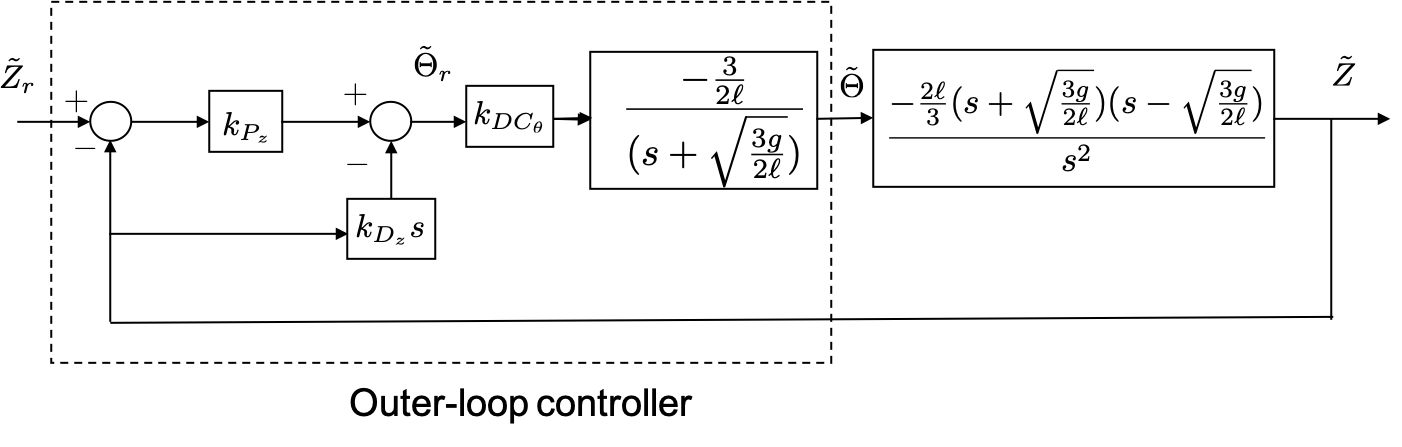
\includegraphics[width=0.95\textwidth]{6_design_studies/figures/hw_pendulum_PD_outer_w_lpf} 
   	\caption{Block diagram for outer loop of inverted pendulum control, with low-pass filter to cancel the LHP zero.}
   	\label{fig:hw_pendulum_PD_outer_w_lpf}
\end{figure}
%
After accounting for the cancelations introduced by the low-pass filter, the equivalent closed-loop systems is shown in Figure~\ref{fig:hw_pendulum_PD_outer_eq}.
\begin{figure}[htbp]
   	\centering
   	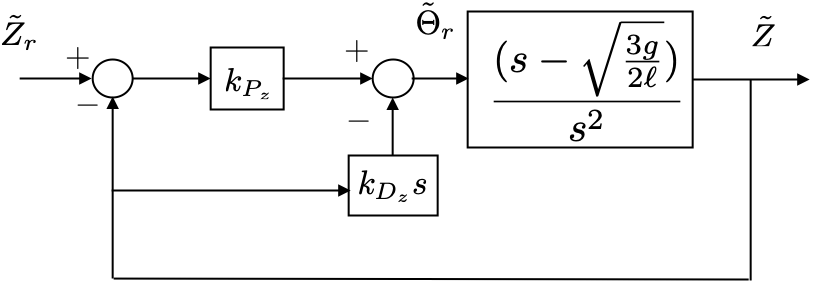
\includegraphics[width=0.6\textwidth]{6_design_studies/figures/hw_pendulum_PD_outer_eq} 
   	\caption{Block diagram for the equivalent outer loop of inverted pendulum control with low-pass filter.}
   	\label{fig:hw_pendulum_PD_outer_eq}
\end{figure}
%
In this case, the closed-loop characteristic equation from $\tilde{Z}_r$ to $\tilde{Z}$ is given by
\[
\tilde{Z}(s) = \left( 
		\frac{\left(\frac{k_{p_z}}{1+k_{d_z}}\right) (s-\sqrt{\frac{3g}{2\ell}})}
		     {s^2 - \left(\frac{k_{p_z} - k_{d_z}\sqrt{\frac{3g}{2\ell}}}{1+k_{d_z}}\right)s - \frac{k_{p_z}\sqrt{\frac{3g}{2\ell}}}{1+k_{d_z}}} 
       \right) \tilde{Z}_r.
\]
Setting the closed-loop characteristic equation equal to the desire closed-loop characteristic equation in Equation~\eqref{eq:delta_cl_d_pendulum_outer} gives
\begin{align}
\frac{k_{p_z}}{1+k_{d_z}} &= -\omega_{n_z}^2\sqrt{\frac{2\ell}{3g}} \defeq a \\
\frac{k_{d_z}}{1+k_{d_z}} &= \left[\frac{k_{p_z}}{1+k_{d_z}} - 2\zeta_z \omega_{n_z} \right] \sqrt{\frac{2\ell}{3g}} \defeq b. 
\end{align}
Then 
\begin{align*}
k_{d_z} &= \frac{b}{1-b} \\
k_{p_z} &= a(1+k_{d_z}).
\end{align*}


A Python class that implements a PD controller for the inverted pendulum is shown below.
\lstinputlisting[language=Python, caption=pendulumController.py]{../control_book_public_solutions/_B_pendulum/python/hw8/pendulumController.py}

Python code that implements the closed loop system is given below.
\lstinputlisting[language=Matlab, caption=pendulumSim.py]{../control_book_public_solutions/_B_pendulum/python/hw8/pendulumSim.py}

Complete simulation code for Matlab, Python, and Simulink can be downloaded at \controlbookurl{http://controlbook.byu.edu}.
